\documentclass[8pt]{beamer}
\usepackage[T1]{fontenc}
\usepackage[francais]{babel}
\usepackage{xcolor}
\usepackage{tikz}
\usetikzlibrary{arrows,shapes,tikzmark,fit}
\usepackage{pslatex}
\usepackage{textcomp}
\usepackage[utf8]{inputenc}
\usepackage{wrapfig}
\usepackage{graphicx}
\usepackage[section]{placeins}
\usepackage{lscape}
\usepackage{float}
\usepackage{amssymb}
\usepackage{wasysym}
\usepackage{pgf}
\usepackage{alltt}
\usepackage{eso-pic}
\usepackage{comment}
\usepackage{ulem}
\usepackage{multirow}

%\usepackage{colortbl}
%\usepackage{pstricks}

\definecolor{MyGray}{gray}{0.85}
\definecolor{MyGreen}{HTML}{31B404}

\newcommand{\refarticle}[2]{\textit{#1} ~~ \fcolorbox{red}{white}{{\tt #2}}}
\newcommand{\crefarticle}[2]{\begin{center}\textit{#1} ~~ \fcolorbox{red}{white}{{\tt #2}} \end{center}}

\usetheme{Frankfurt}

\graphicspath{{figs/}}

\title[Séminaire 2ieme année]{Développement d'un algorithme de suivi \\ de particules (PFA) pour l'ILC. Outils de surveillance \\ en ligne de qualité de données}
\institute{\normalsize Institut de Physique Nucléaire de Lyon}
\author[R. Eté]{{\large \bf Rémi \'ET\'E} \\ {\bf Directeur de thèse : Imad LAKTINEH}}
\date{8 mars 2017}

\DeclareUnicodeCharacter{00A0}{ }

\setbeamertemplate{itemize items}[ball]
%\addtobeamertemplate{block begin}{\pgfsetfillopacity{0.5}}{\pgfsetfillopacity{1}}

\begin{document}

  %%%%%%%%%%%%%% Page de présentation %%%%%%%%%%%%%%
  \begin{frame}
    \titlepage
    \begin{center}
      
\includegraphics[width=0.2\textwidth]{logo/logo_ipnl.jpg} ~~~
      
\includegraphics[width=0.2\textwidth]{logo/logo-univ-lyon.png} ~~~
      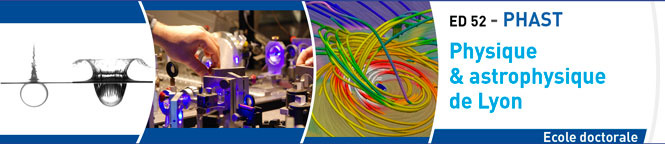
\includegraphics[width=0.5\textwidth]{logo/logo-edphast.jpg}
    \end{center}
  \end{frame}


  \begin{frame}
  \frametitle{Sommaire}
    \tableofcontents
  \end{frame}

%%%%%%%%%%%%%%%%%%
%% INTRODUCTION %%
%%%%%%%%%%%%%%%%%%

  \section{Introduction}

  \begin{frame}
  \frametitle{\secname}
    \tableofcontents[currentsection]
  \end{frame}

  \subsection{Le modèle standard}

  %% Modele standard
  \begin{frame}
  \frametitle{\secname}
  \framesubtitle{Le modèle standard}
    \begin{minipage}{0.6\linewidth}
      \begin{block}{Le modèle standard}
        Théorie unifiant 3 des 4 interactions fondamentales :
        \begin{itemize}
          \item L'interaction électromagnétique
          \item L'interaction faible
          \item L'interaction forte
        \end{itemize}
        Théorie de jauge SU(3) $\bigotimes$ SU(2) $\bigotimes$ U(1)
      \end{block}
    \end{minipage} \hfill
    \begin{minipage}{0.38\linewidth}
      \begin{tikzpicture}
        \node[anchor=south west,inner sep=0] at (0,0) {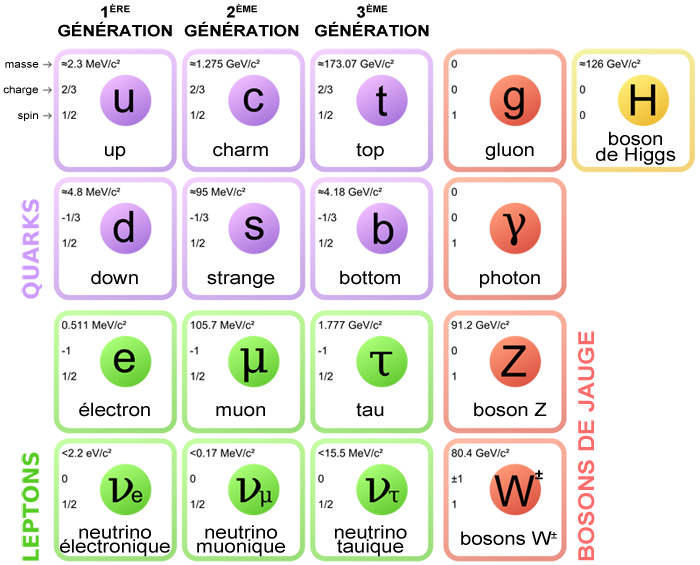
\includegraphics[width=0.9\linewidth]{figs/Particules_elementaires.png}};
        \draw<2>[red, thick, overlay] (3.03,2.1) rectangle (3.65,2.7);
        % \draw<2>[red, thick, overlay, ->] (3.65,2.4) -- (4,2.4) -- (4,0.5);
      \end{tikzpicture}
      % 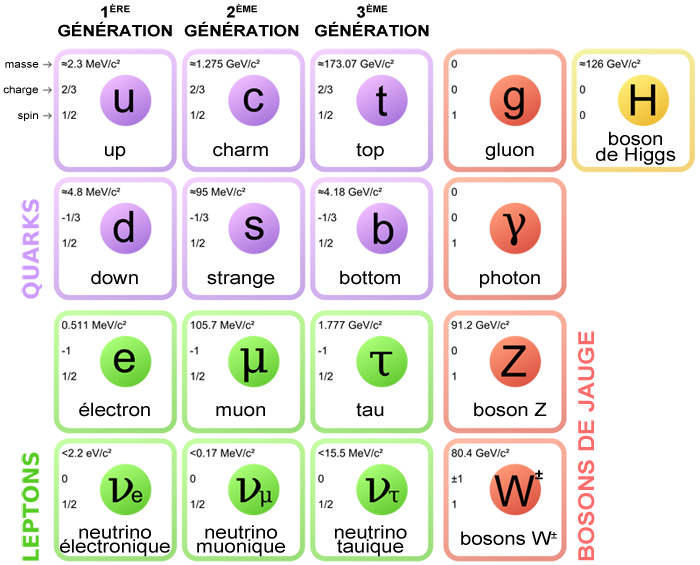
\includegraphics[width=0.9\linewidth]{figs/Particules_elementaires.png}
    \end{minipage}
    \begin{minipage}{0.48\linewidth}
      \begin{tikzpicture}
        \node[anchor=south west,inner sep=0] at (0,0) {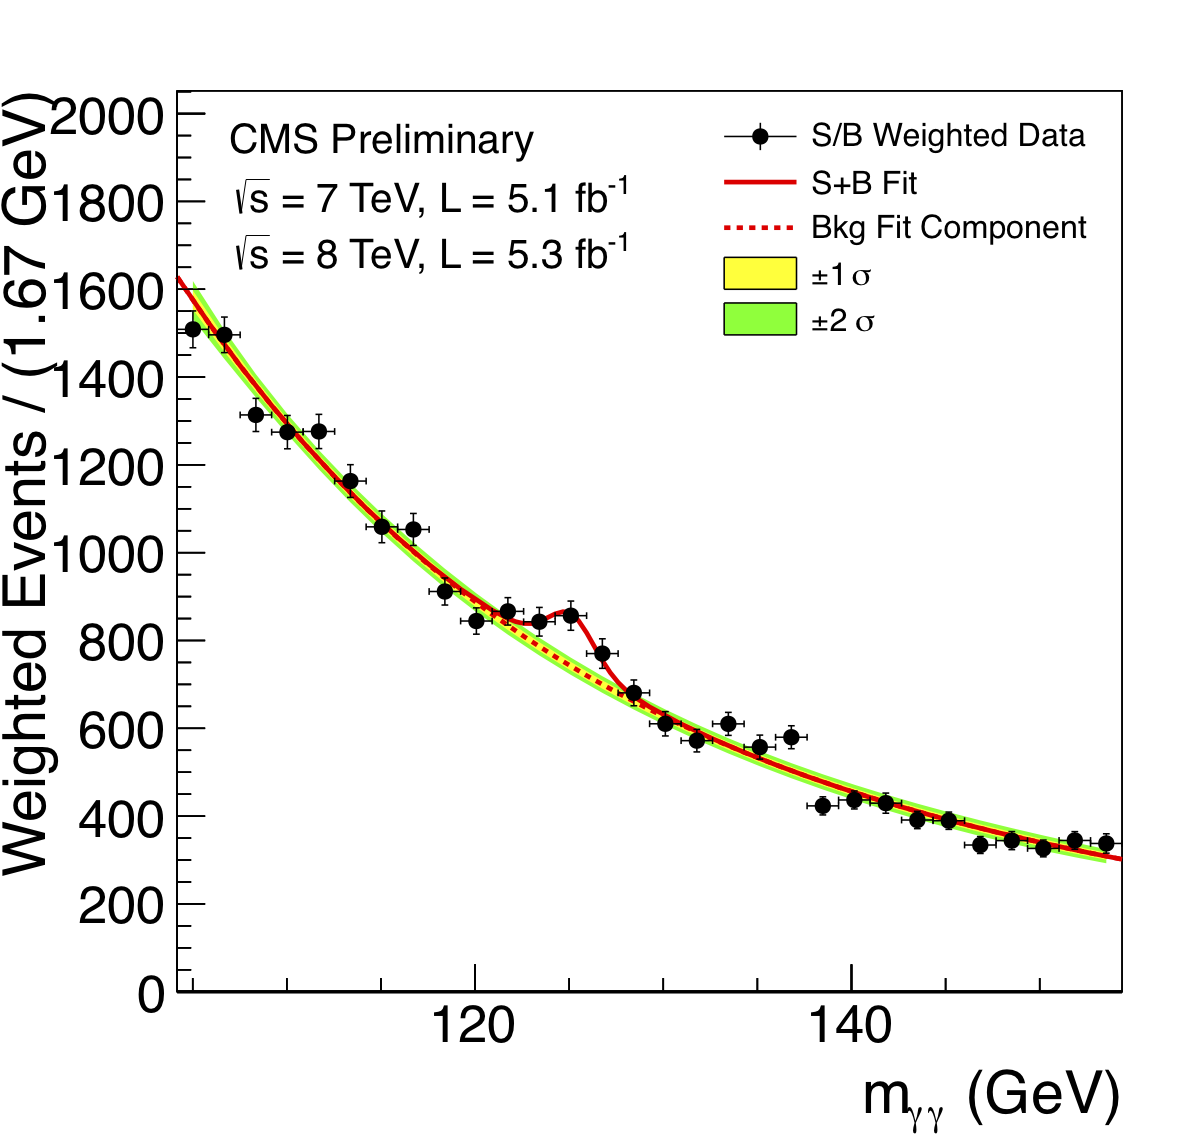
\includegraphics[width=0.9\linewidth]{figs/CMS_Higgs_plot.png}};
        \draw<2>[red, thick, overlay] (2.3,2) circle (0.4);
      \end{tikzpicture}
      % 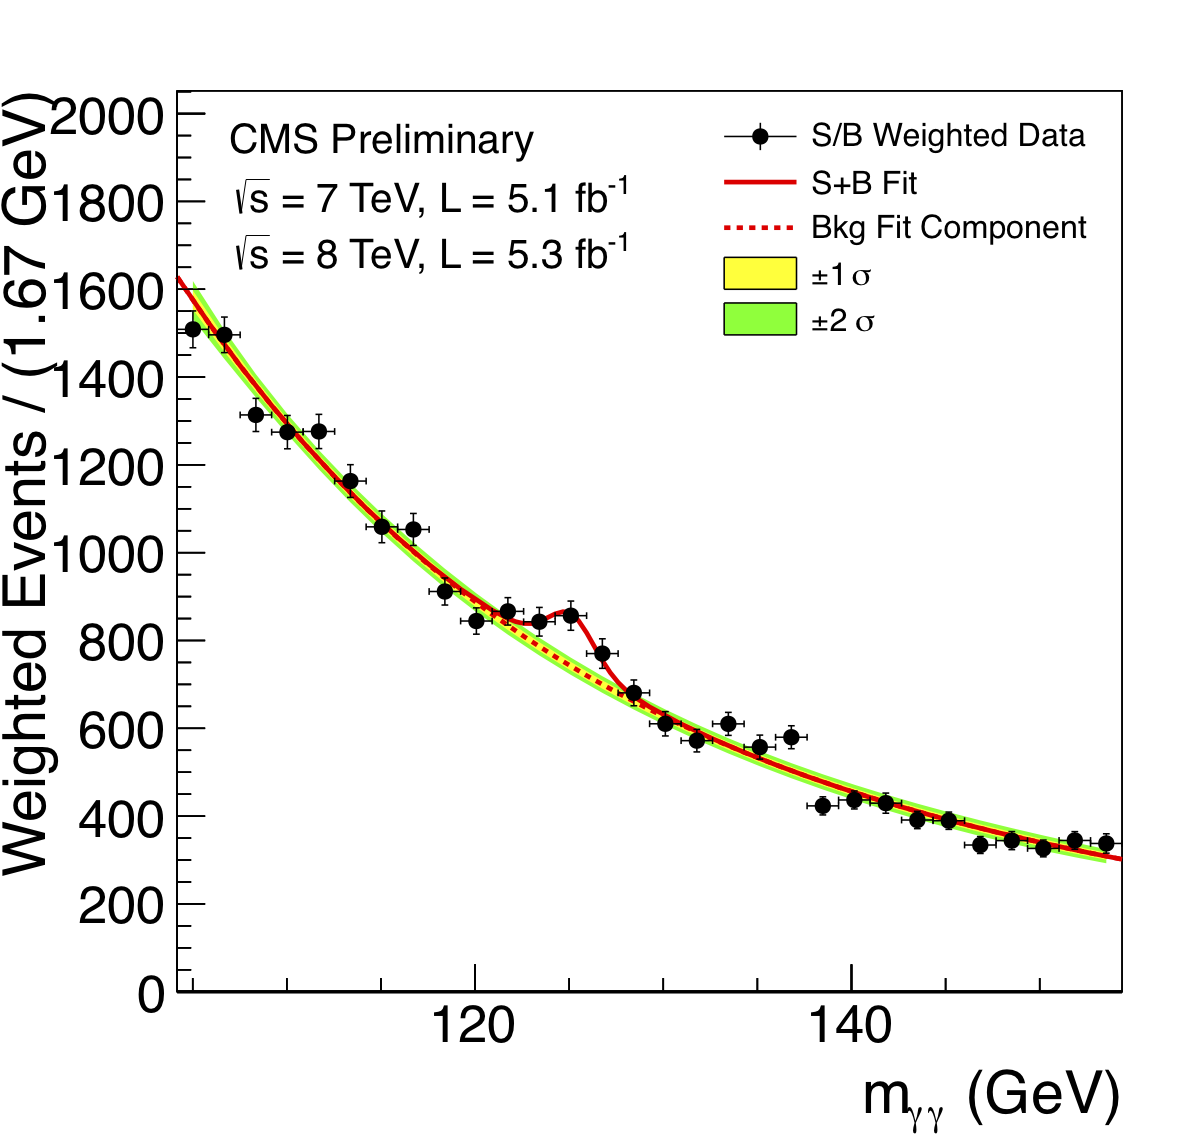
\includegraphics[width=0.9\linewidth]{figs/CMS_Higgs_plot.png}
    \end{minipage}
    \begin{minipage}{0.48\linewidth}
      \begin{block}{Des familles et des générations !}
        \begin{itemize}
          \item 12 fermions
          \item 4 bosons de jauge
          \item 1 boson de Higgs
        \end{itemize}
      \end{block}
      \begin{block}{Modèle incomplet}
        \begin{itemize}
          \item Pas de gravitation
          \item Masse/oscillation neutrinos
          \item Asymétrie matière/anti-matière
        \end{itemize}
      \end{block}
    \end{minipage}
    \begin{tikzpicture}
      \draw<2>[red, thick, overlay, ->] (-0.18,4.75) -- (0.3,4.75) -- (0.3,-2.2) -- (-8.25,-2.2) -- (-8.25,-0.6);
    \end{tikzpicture}
  \end{frame}


  \subsection{Le collisionneur linéaire international}

  %% L'ILC
  \begin{frame}
  \frametitle{\secname}
  \framesubtitle{Le collisionneur linéaire international - ILC}
    \begin{center}
      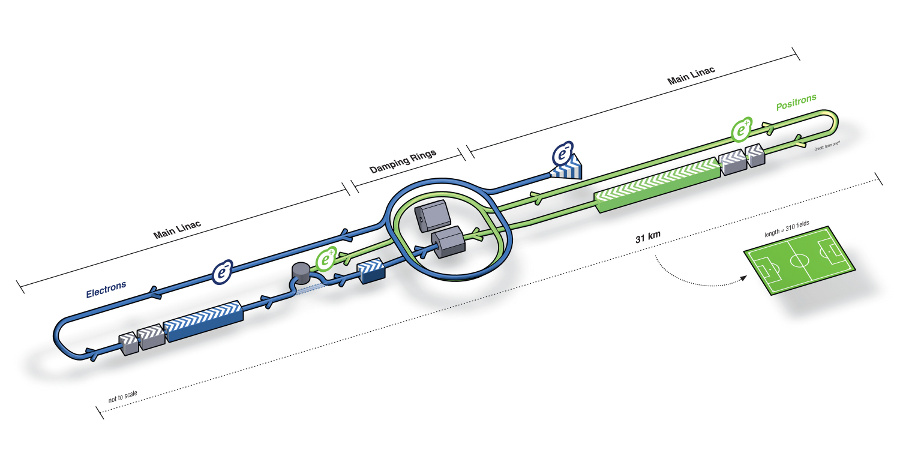
\includegraphics[width=0.55\linewidth]{figs/ilc_layout.jpg}
    \end{center}
    \begin{minipage}{0.51\linewidth}
      \begin{block}{Caractéristiques du collisionneur}
        \begin{itemize}
          \item Collision e$^{+}$ e$^{-}$
          \item Energie : 250-500 GeV (1 TeV ?)
          \item Luminosité : 0.75$\cdot$10$^{34}$-1.8$\cdot$10$^{34}$ cm$^{-2}$s$^{-1}$
          \item Fréquence de collisions : 5 Hz (contre 40 MHz au LHC)
          \item Nb de particules par croisement : 2 $\cdot$ 10$^{10}$
          \item Alimentation pulsée
        \end{itemize}
      \end{block}
    \end{minipage} \hfill
    \begin{minipage}{0.46\linewidth}
      \begin{tikzpicture}
        \node[anchor=south west,inner sep=0] at (0,0) {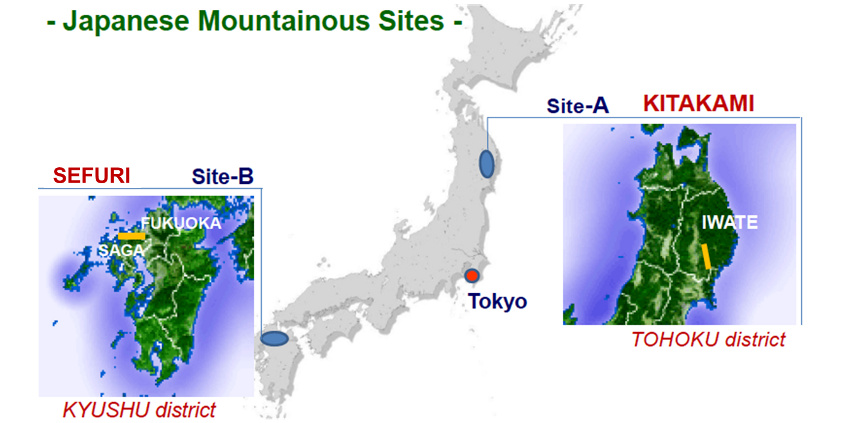
\includegraphics[width=\linewidth]{figs/japanese_sites.jpg}};
        \draw<2>[red, thick, overlay] (3.7,1.3) circle (1.4);
      \end{tikzpicture}
      \crefarticle{ILC Technical Design Report, \\Vol.1 Executive Summary \\}{arXiv:1306.6327}
      % \begin{center}  {\tt } \end{center}
    \end{minipage}
  \end{frame}

  %% Le programme de l'ILC
  \begin{frame}
  \frametitle{\secname}
  \framesubtitle{Le programme physique}
    \begin{center}
      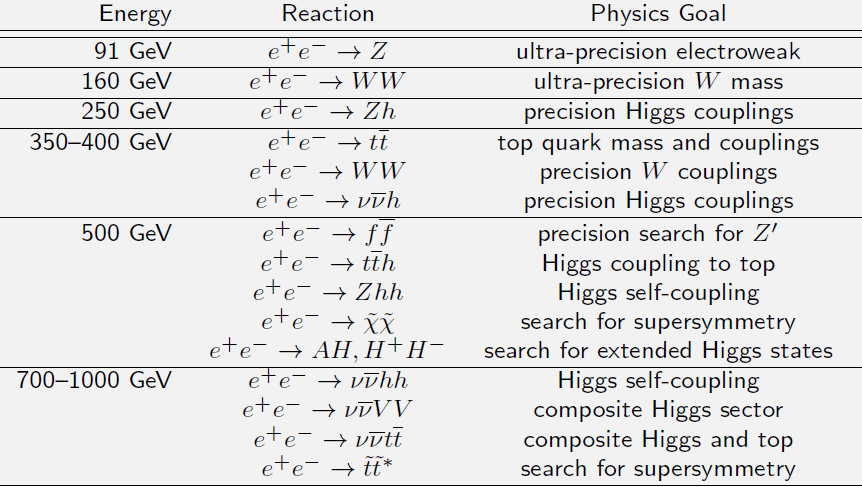
\includegraphics[width=\linewidth]{figs/ilc_program.png}
    \end{center}
    \crefarticle{ILC Technical Design Report, Vol.2 : Physics}{arXiv:1306.6352}
  \end{frame}

  %% ILD et SiD
  \begin{frame}
  \frametitle{\secname}
  \framesubtitle{ILD et SiD}
    \begin{minipage}{0.54\linewidth}
      Deux détecteurs génériques :
      \begin{itemize}
        \item ILD : TPC, plus large, B = 3.5 - 4 T
        \item SiD : Tracker en silicium, plus compact, B = 5 T
      \end{itemize}
      ~ \\
      Installation sur rail coulissant \\
      \crefarticle{ILC Technical Design Report, Vol.4 Detectors \\}{arXiv:1306.6329}
    \end{minipage}
    \begin{minipage}{0.45\linewidth}
      \begin{center}
        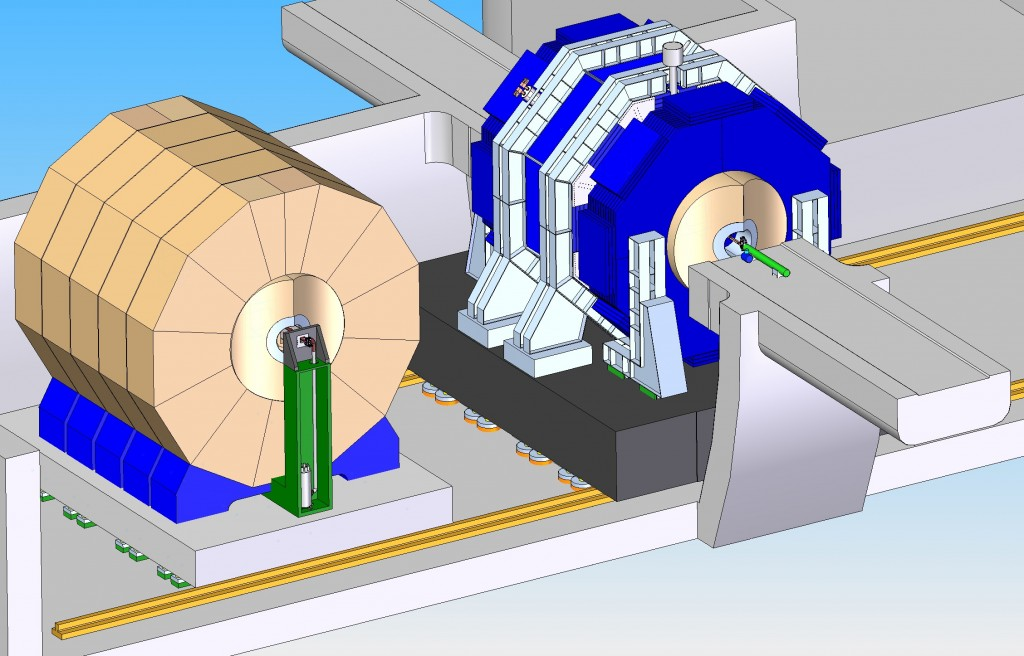
\includegraphics[width=0.94\linewidth]{figs/ild_sid.jpg}
      \end{center}
    \end{minipage}
    ~ \\
    ~ \\
    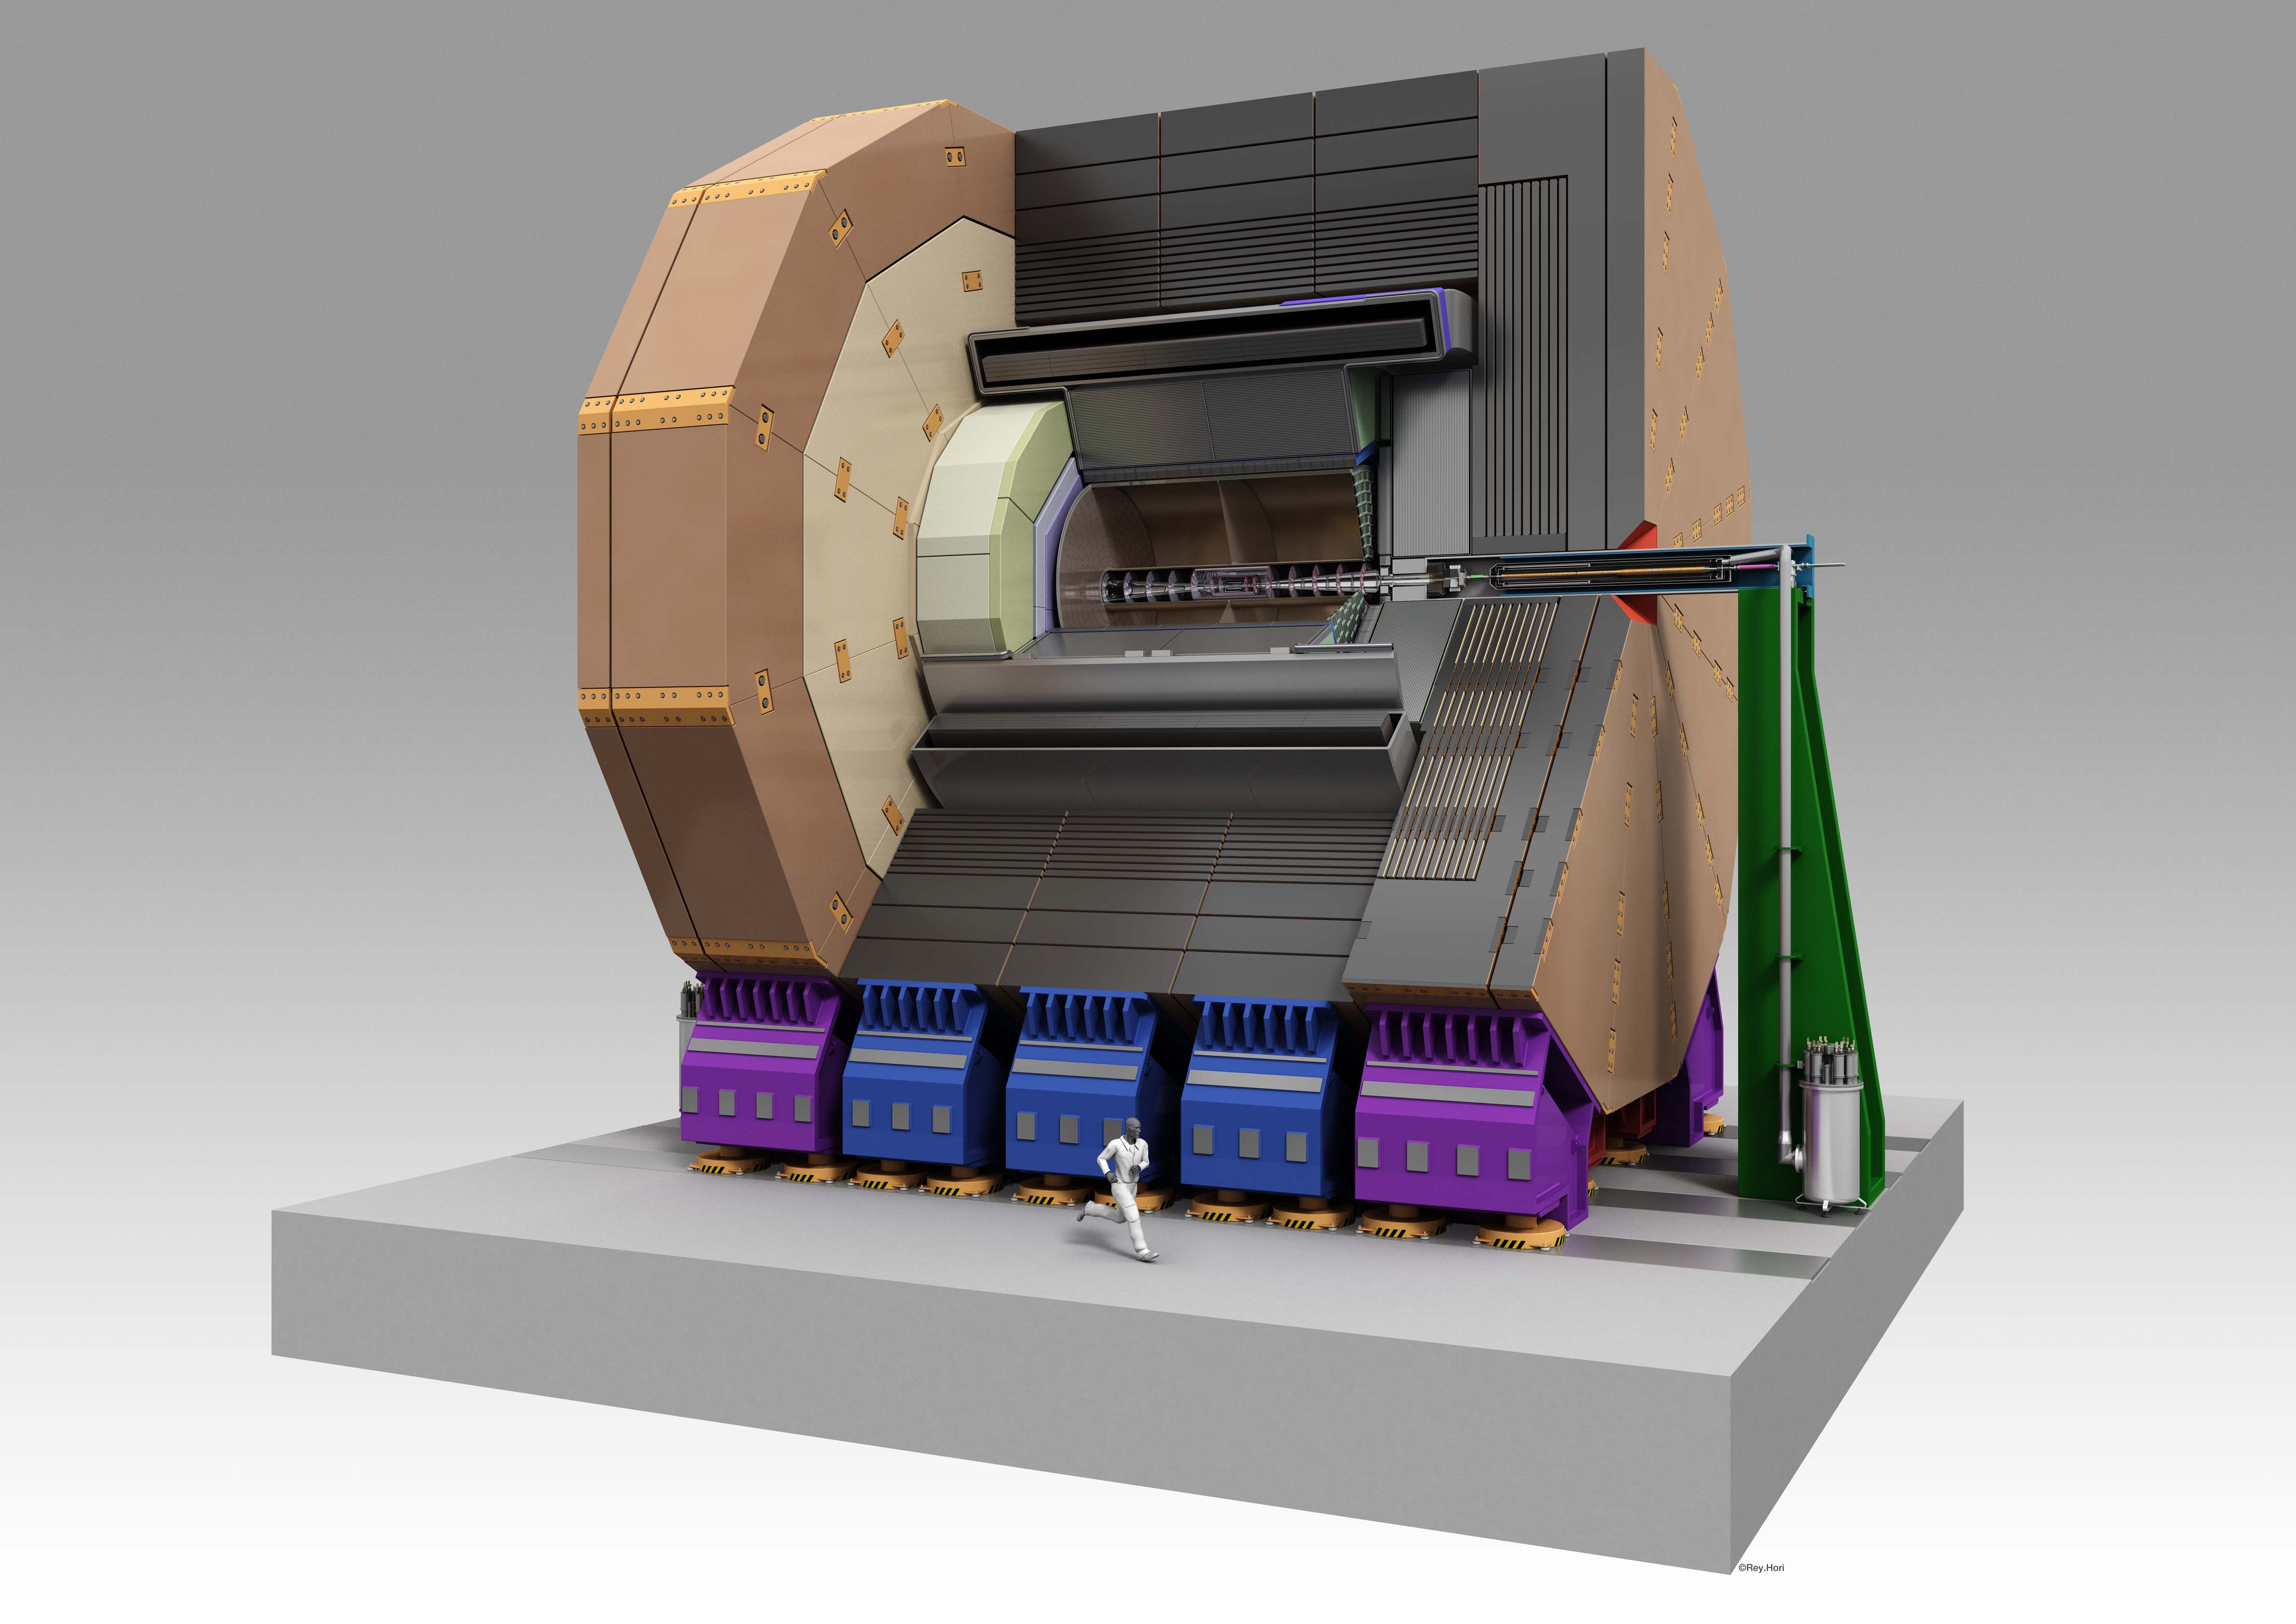
\includegraphics[width=0.48\linewidth]{figs/ild.jpg} ~~~~
    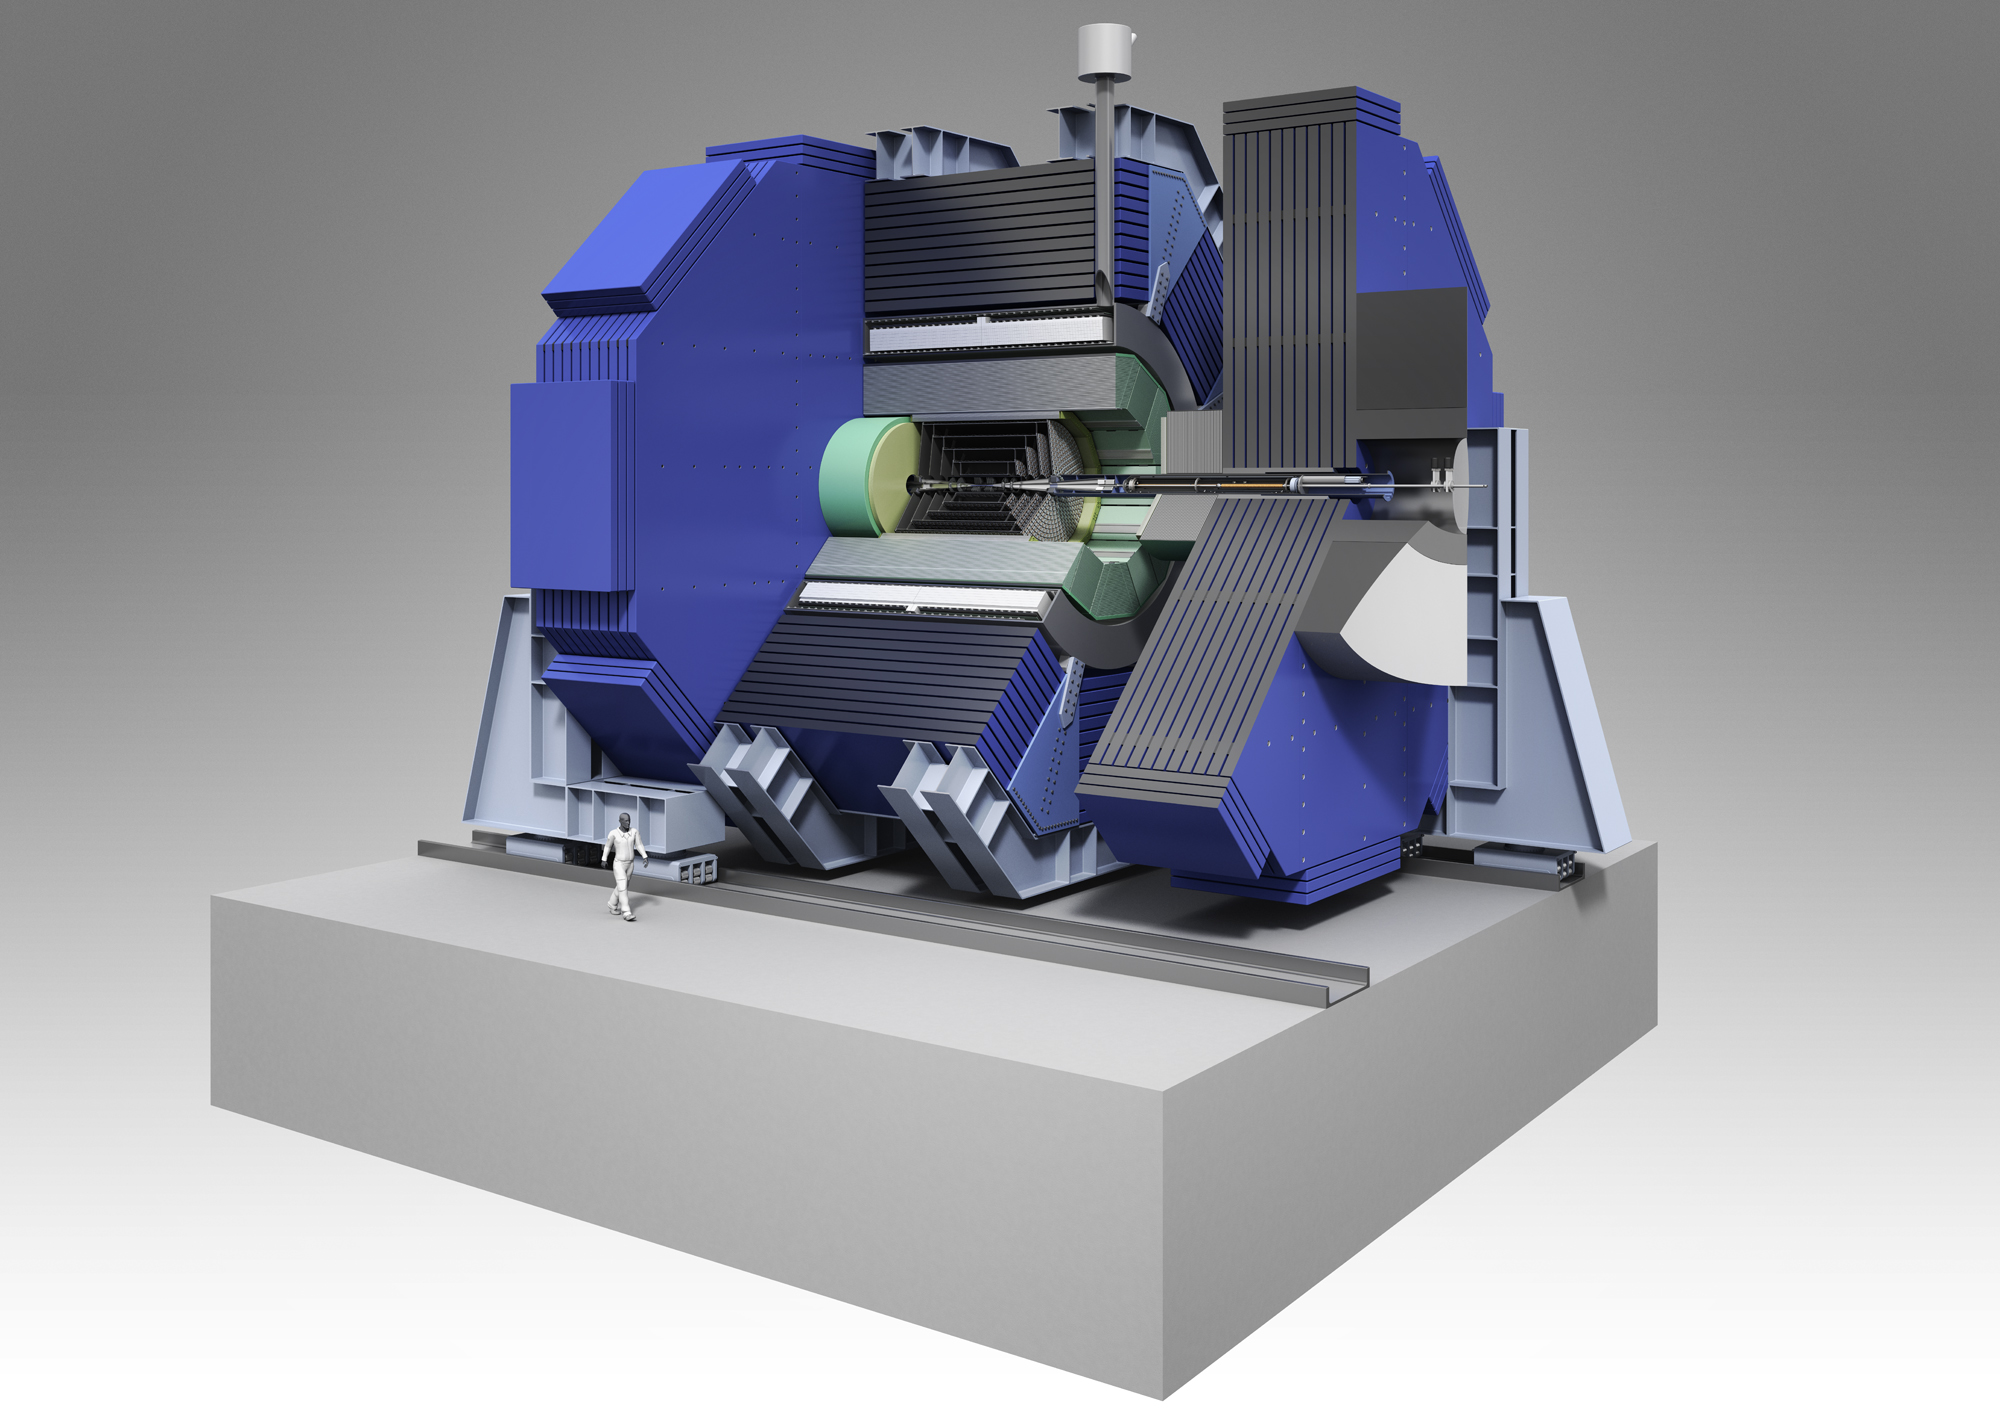
\includegraphics[width=0.48\linewidth]{figs/sid.jpg}
  \end{frame}


  %% Les sous détecteurs
  \begin{frame}
  \frametitle{\secname}
  \framesubtitle{Les sous détecteurs de l'ILD}
    \begin{minipage}{0.62\linewidth}
      \begin{table}
        \begin{tabular}{c|c|c}
          \hline
          \multicolumn{1}{c}{Détecteur} & \multicolumn{1}{c}{Mesure} & \multicolumn{1}{c}{Performance} \\ 
          \hline \hline
          Trajectographe & 1 / $\delta_p$                           & 10$^{-5}$ (GeV/c)$^{-1}$ \\
          Tracking + Calo (jet)   & $\frac{\Delta E}{E}$                     & 3-4 \% \\
          \multirow{3}{*}{Vertex}         & {\footnotesize Résolution spatial}       & {\footnotesize < 3 $\mu m$} \\
          ~              & {\footnotesize Budget matière}           & {\footnotesize < 0.15 \% $X_{0}$/layer} \\
          ~              & {\footnotesize Rayon premier layer}      & {\footnotesize $\simeq$ 1.6 $cm$}
        \end{tabular}
      \end{table}
    \end{minipage} \hfill
    \begin{minipage}{0.36\linewidth}
      \begin{tikzpicture}
        \node[anchor=south west,inner sep=0] at (0,0) {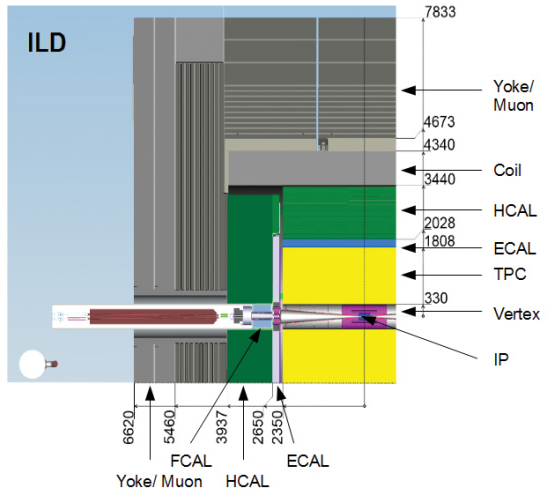
\includegraphics[width=\linewidth]{figs/ild_vue_en_coupe.png}};
        \draw<2>[red,  thick, overlay] (1.95,1.8) -- (2.8,1.8) -- (2.8,2.2) -- (1.6,2.2) -- (1.6,1.4) -- (1.95,1.4) -- (1.95,1.8);
      \end{tikzpicture}
    \end{minipage}
    \begin{minipage}[h]{0.5\linewidth}
      \begin{block}{Des calorimètres pour le suivi de particules}
        \begin{itemize}
          \item ECAL (résolution $\simeq 12\%/\sqrt{E}$) :
          \begin{itemize}
            \item SiWECal : 5 x 5 $mm^2$
            \item ScWECal : 5 x 45 $mm^2$ + SSA
          \end{itemize}
          \item HCAL (résolution $\simeq 60\%/\sqrt{E}$) :
          \begin{itemize}
            \item AHCAL : 3 x 3 $cm^2$
            \item SDHCAL : 1 x 1 $cm^2$
          \end{itemize}
        \end{itemize}
      \end{block}
      \crefarticle{ILC Technical Design Report, Vol.4 Detectors \\}{arXiv:1306.6329}
    \end{minipage} \hfill
    \begin{minipage}[h]{0.48\linewidth}
      \begin{tikzpicture}
        \node[anchor=south west,inner sep=0] at (0,0) {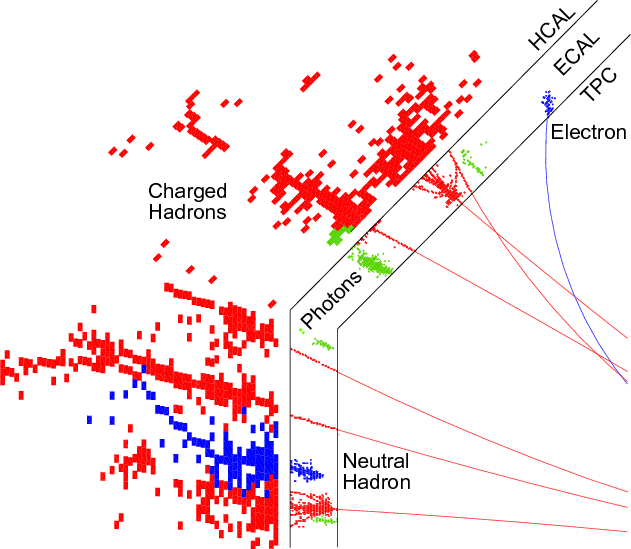
\includegraphics[width=0.8\linewidth]{figs/pfa_event_display.png}};
        \draw<2>[red,  thick, overlay] (1.9,1.6) -- (1.9,0) -- (0,0) -- (0,3.62) -- (3.9,3.62) -- (1.9,1.6);
      \end{tikzpicture}
    \end{minipage}
  \end{frame}

  %% Le prototype SDHCAL
  \subsection{Le calorimètre hadronique semi-digital}

  \begin{frame}
  \frametitle{\secname}
  \framesubtitle{\subsecname}
    \begin{minipage}{0.52\linewidth}
      \begin{block}{Semi-Digital Hadron Calorimeter}
        \begin{itemize}
          \item Calorimètre à échantillonnage
          \item 48 plans :
          \begin{itemize}
            \item Absorber en acier
            \item Milieu sensitif : GRPC
          \end{itemize}
          \item Segmentation :
          \begin{itemize}
            \item Transverse : 1 $cm^2$
            \item Longitudinale : 2.67 cm (abs. + sens)
          \end{itemize}
          \item Lecture semi-digitale à 3 seuils
          \begin{itemize}
            \item \textcolor{MyGreen}{seuil 1} : peu de particules
            \item \textcolor{blue}{seuil 2} : quelques particules
            \item \textcolor{red}{seuil 3} : beaucoup de particules
          \end{itemize}
        \end{itemize}
      \end{block}
      \crefarticle{The Calice Collaboration}{arXiv:1602.02276}
    \end{minipage} \hfill
    \begin{minipage}{0.46\linewidth}
      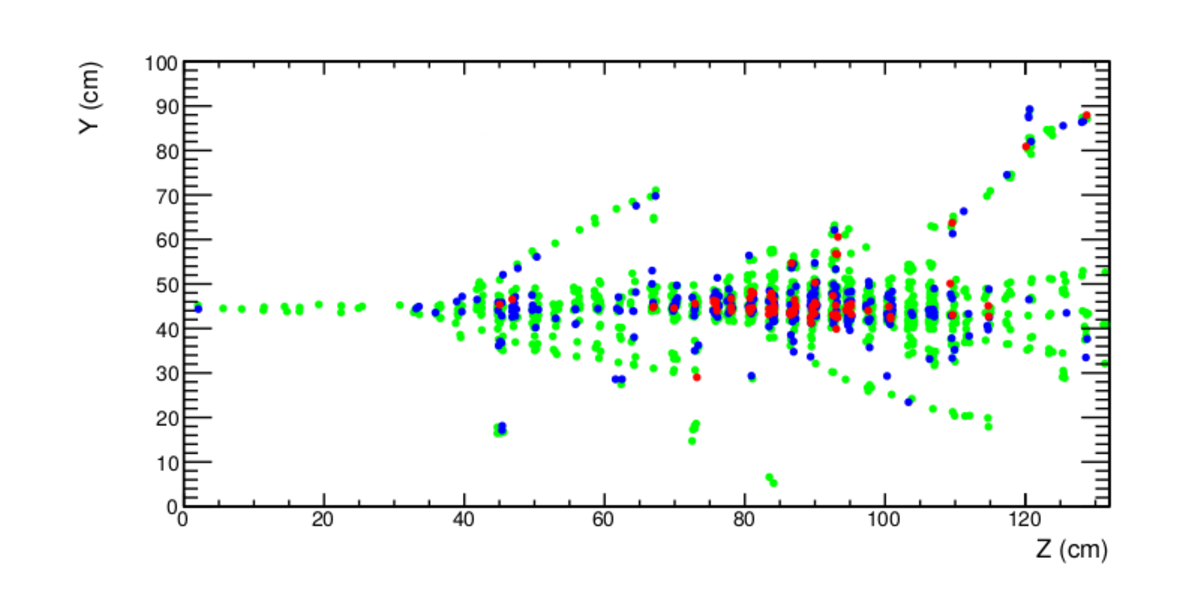
\includegraphics[width=\linewidth]{figs/sdhcal_pion_80GeV.pdf}
    \end{minipage}
    \begin{minipage}{0.58\linewidth}
      \begin{center}
        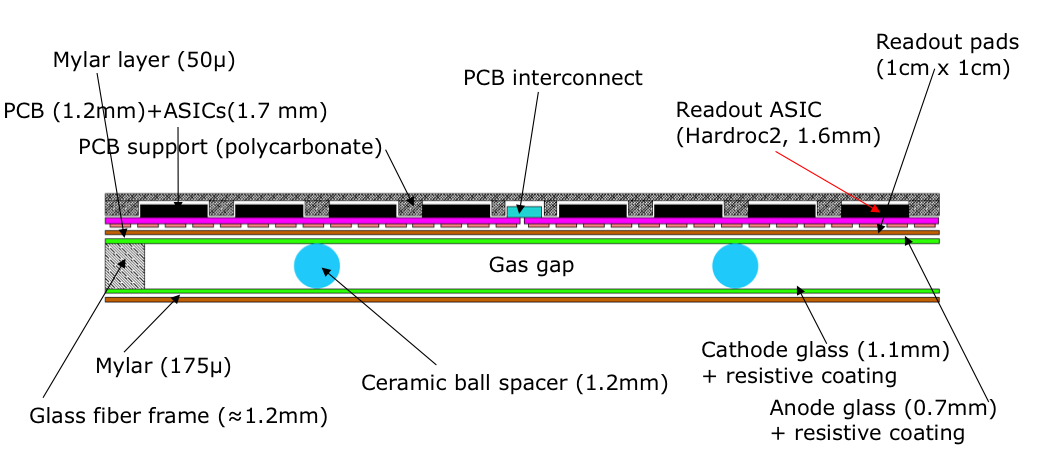
\includegraphics[width=0.9\linewidth]{figs/GRPC-K7.png}
      \end{center}
    \end{minipage} \hfill
    \begin{minipage}{0.4\linewidth}
      \begin{center}
        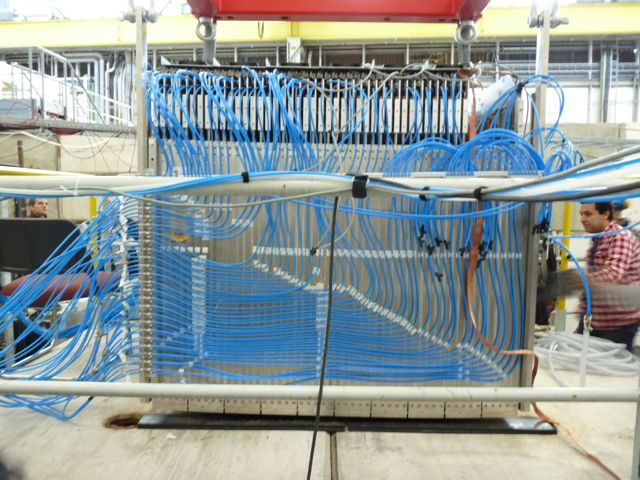
\includegraphics[width=0.7\linewidth]{figs/sdhcal_testbeam.jpg}
      \end{center}
    \end{minipage}
  \end{frame}


  %% Performances du SDHCAL
  \subsection{Performances du SDHCAL}

  %% Multiplicité / Efficacité
  \begin{frame}
  \frametitle{\secname}
  \framesubtitle{\subsecname}
    \begin{minipage}{0.5\linewidth}
      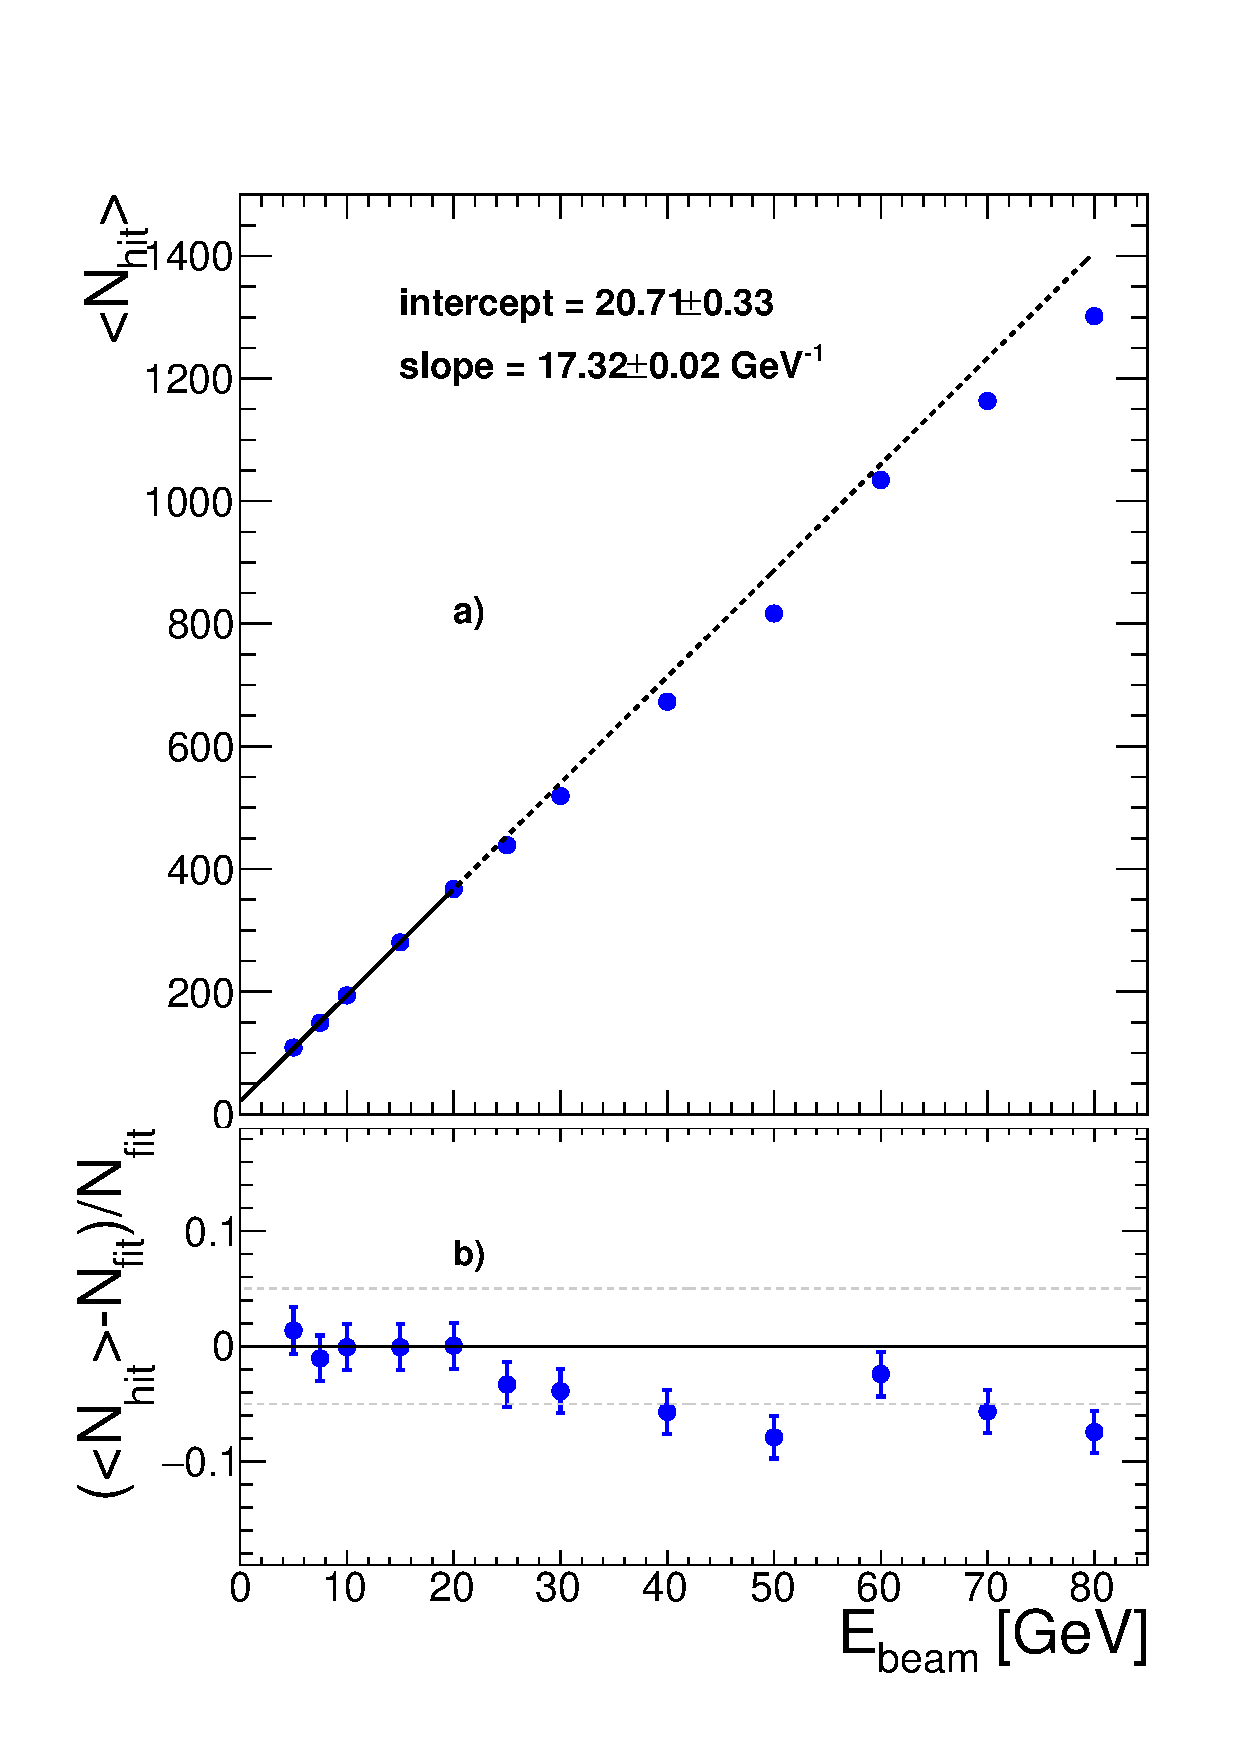
\includegraphics[width=1\linewidth]{figs/NHITPION.pdf}
    \end{minipage} \hfill
    \begin{minipage}{0.48\linewidth}
      \begin{center}
        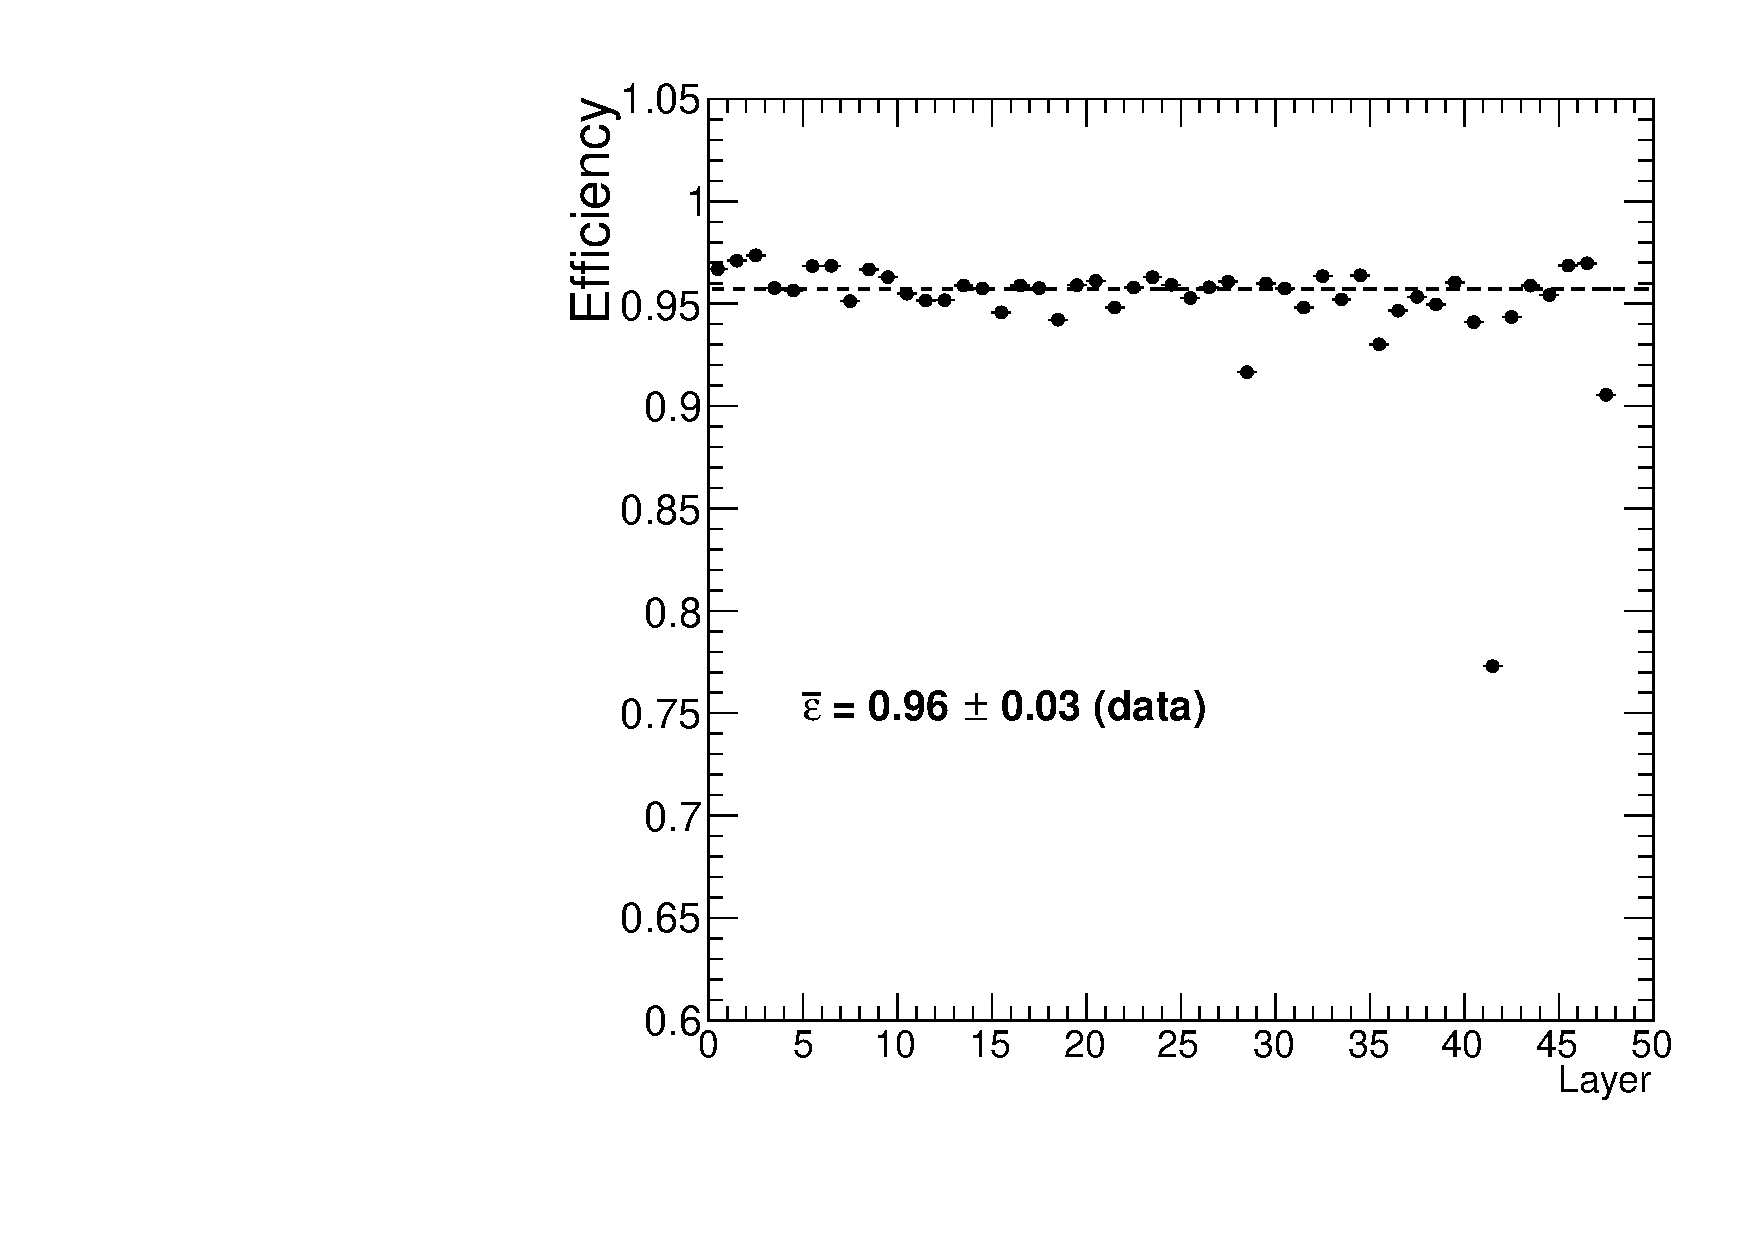
\includegraphics[width=0.7\linewidth]{figs/eff_2012.pdf} \\
        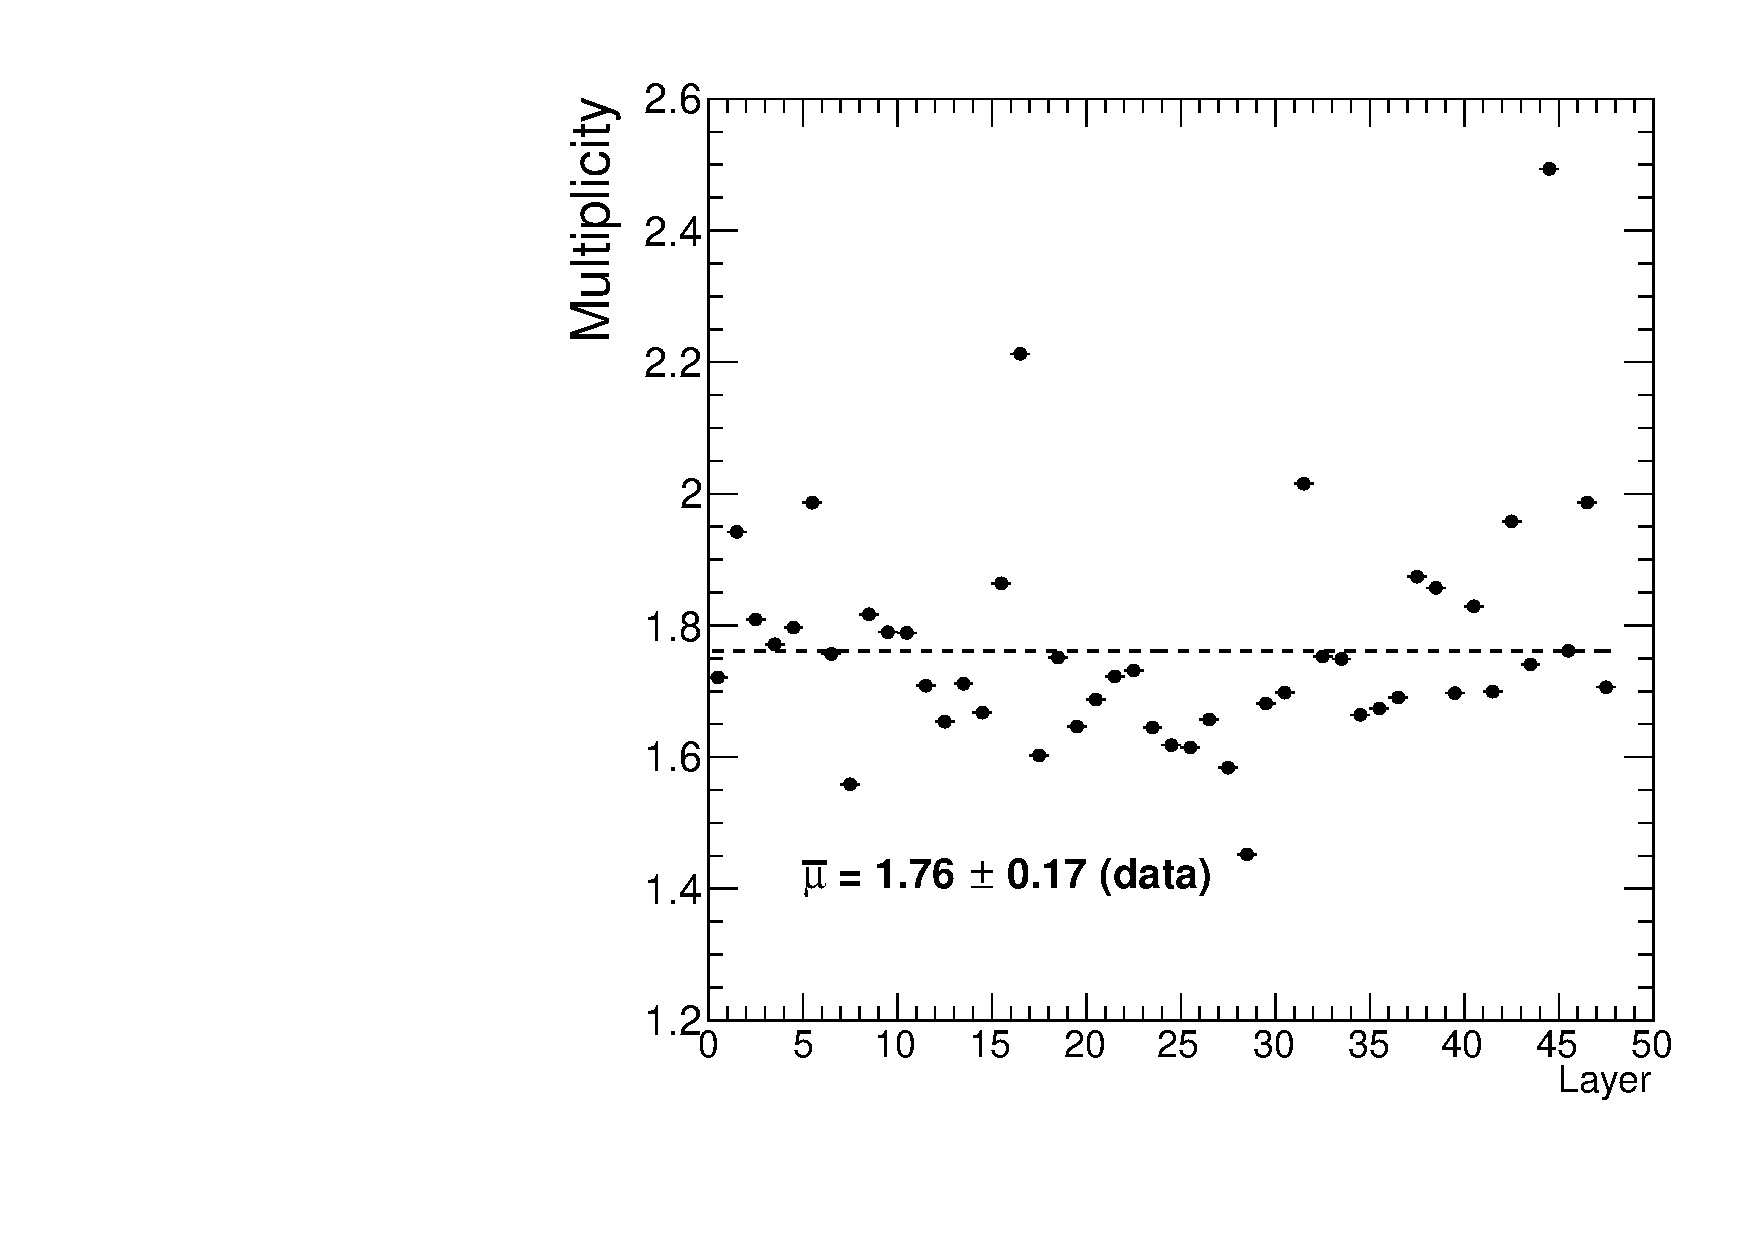
\includegraphics[width=0.7\linewidth]{figs/mul_2012.pdf}
      \end{center}
    \end{minipage}
    \crefarticle{The Calice Collaboration}{arXiv:1604.04550}
  \end{frame}


  %% Reconstruction de l'énergie
  \begingroup
  \small
  \begin{frame}
  \frametitle{\secname}
  \framesubtitle{\subsecname}

    \begin{minipage}{0.65\linewidth}

      Principales observables du SDHCAL : $N_{hit}$, \textcolor{MyGreen}{$N_1$}, \textcolor{blue}{$N_2$}, \textcolor{red}{$N_3$} \\

      Reconstruction de l'énergie des hadrons : \\
      $\rightarrow$ plusieurs estimateurs possibles !

      \pause
      \begin{block}{Formule linéaire}
        \begin{equation}
          E = \alpha\cdot \textcolor{MyGreen}{N_1} + \beta\cdot \textcolor{blue}{N_2} + \gamma\cdot \textcolor{red}{N_3}
        \end{equation}
        avec $\alpha$, $\beta$ et $\gamma$ trois constantes.
        \begin{itemize}
          \item[\textcolor{MyGreen}{$\checkmark$}] Application très simple aux techniques de \textit{PFA}
          \item[\textcolor{red}{$\times$}] Mauvaise linéarité à basse énergie
        \end{itemize}
      \end{block}

      \pause
      \begin{block}{Formule quadratique}
        \begin{equation}
          E = \alpha(NHit)\cdot \textcolor{MyGreen}{N_1} + \beta(NHit)\cdot \textcolor{blue}{N_2} + \gamma(NHit)\cdot \textcolor{red}{N_3}
        \end{equation}
        avec :
        \begin{equation}
          \alpha(NHit) = \alpha_1 + \alpha_2\cdot NHit + \alpha_3\cdot NHit^2
        \end{equation}
        \begin{equation}
          \beta(NHit) = \beta_1 + \beta_2\cdot NHit + \beta_3\cdot NHit^2
        \end{equation}
        \begin{equation}
          \gamma(NHit) = \gamma_1 + \gamma_2\cdot NHit + \gamma_3\cdot NHit^2
        \end{equation}
        \begin{itemize}
          \item[\textcolor{MyGreen}{$\checkmark$}] Bonne linéarité et résolution sur toute la gamme en énergie
          \item[\textcolor{red}{$\times$}] Application aux techniques de \textit{PFA} plus complexe
        \end{itemize}
      \end{block}

    \end{minipage} \hfill
    \begin{minipage}{0.3\linewidth}

      \pause
      \begin{tikzpicture}
        \draw[red,  thick, overlay] (-7.8,-7.8) rectangle (-0.3,-4);
        \draw[red,  thick, overlay] (-0.1,-7) rectangle (3.5,0);
      \end{tikzpicture}
      \begin{center}
        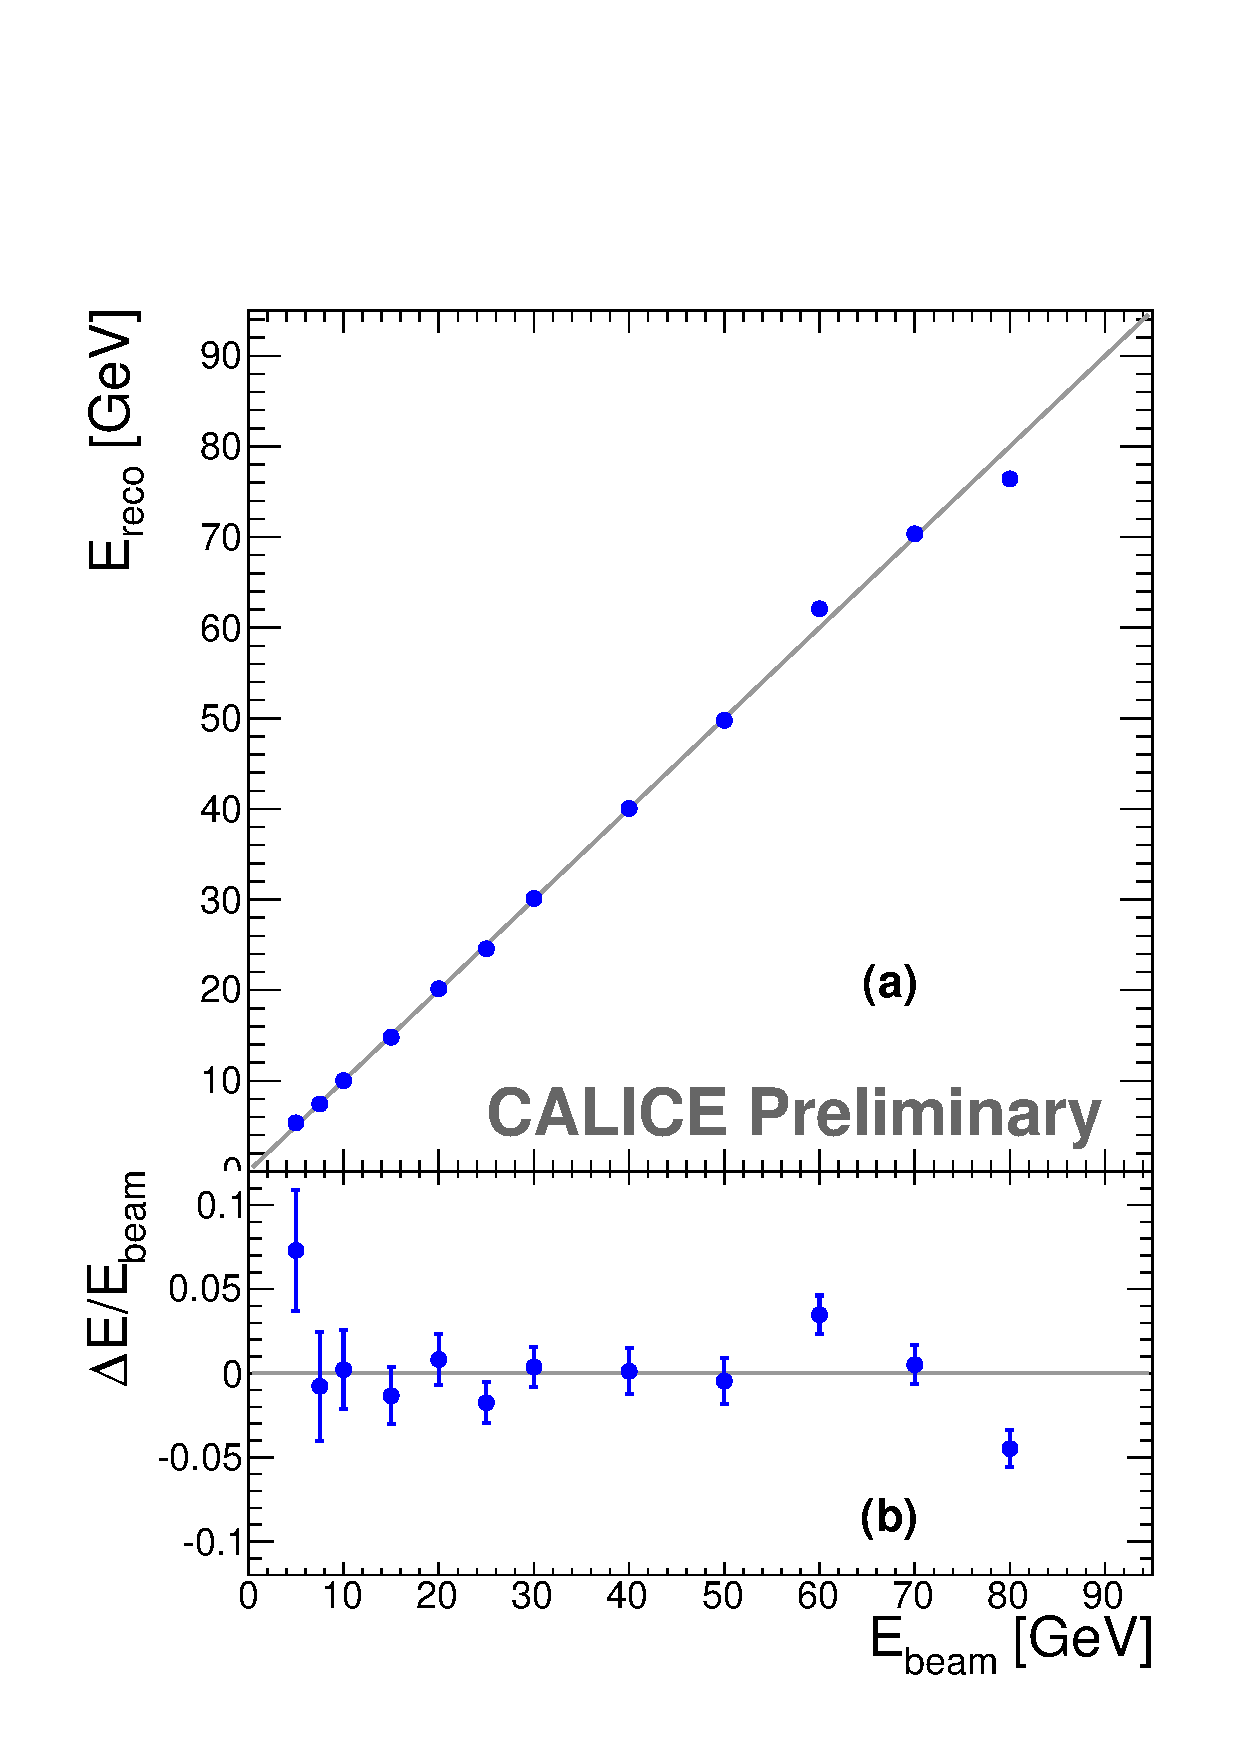
\includegraphics[width=\linewidth]{figs/Energy-Linearity.pdf} \\
        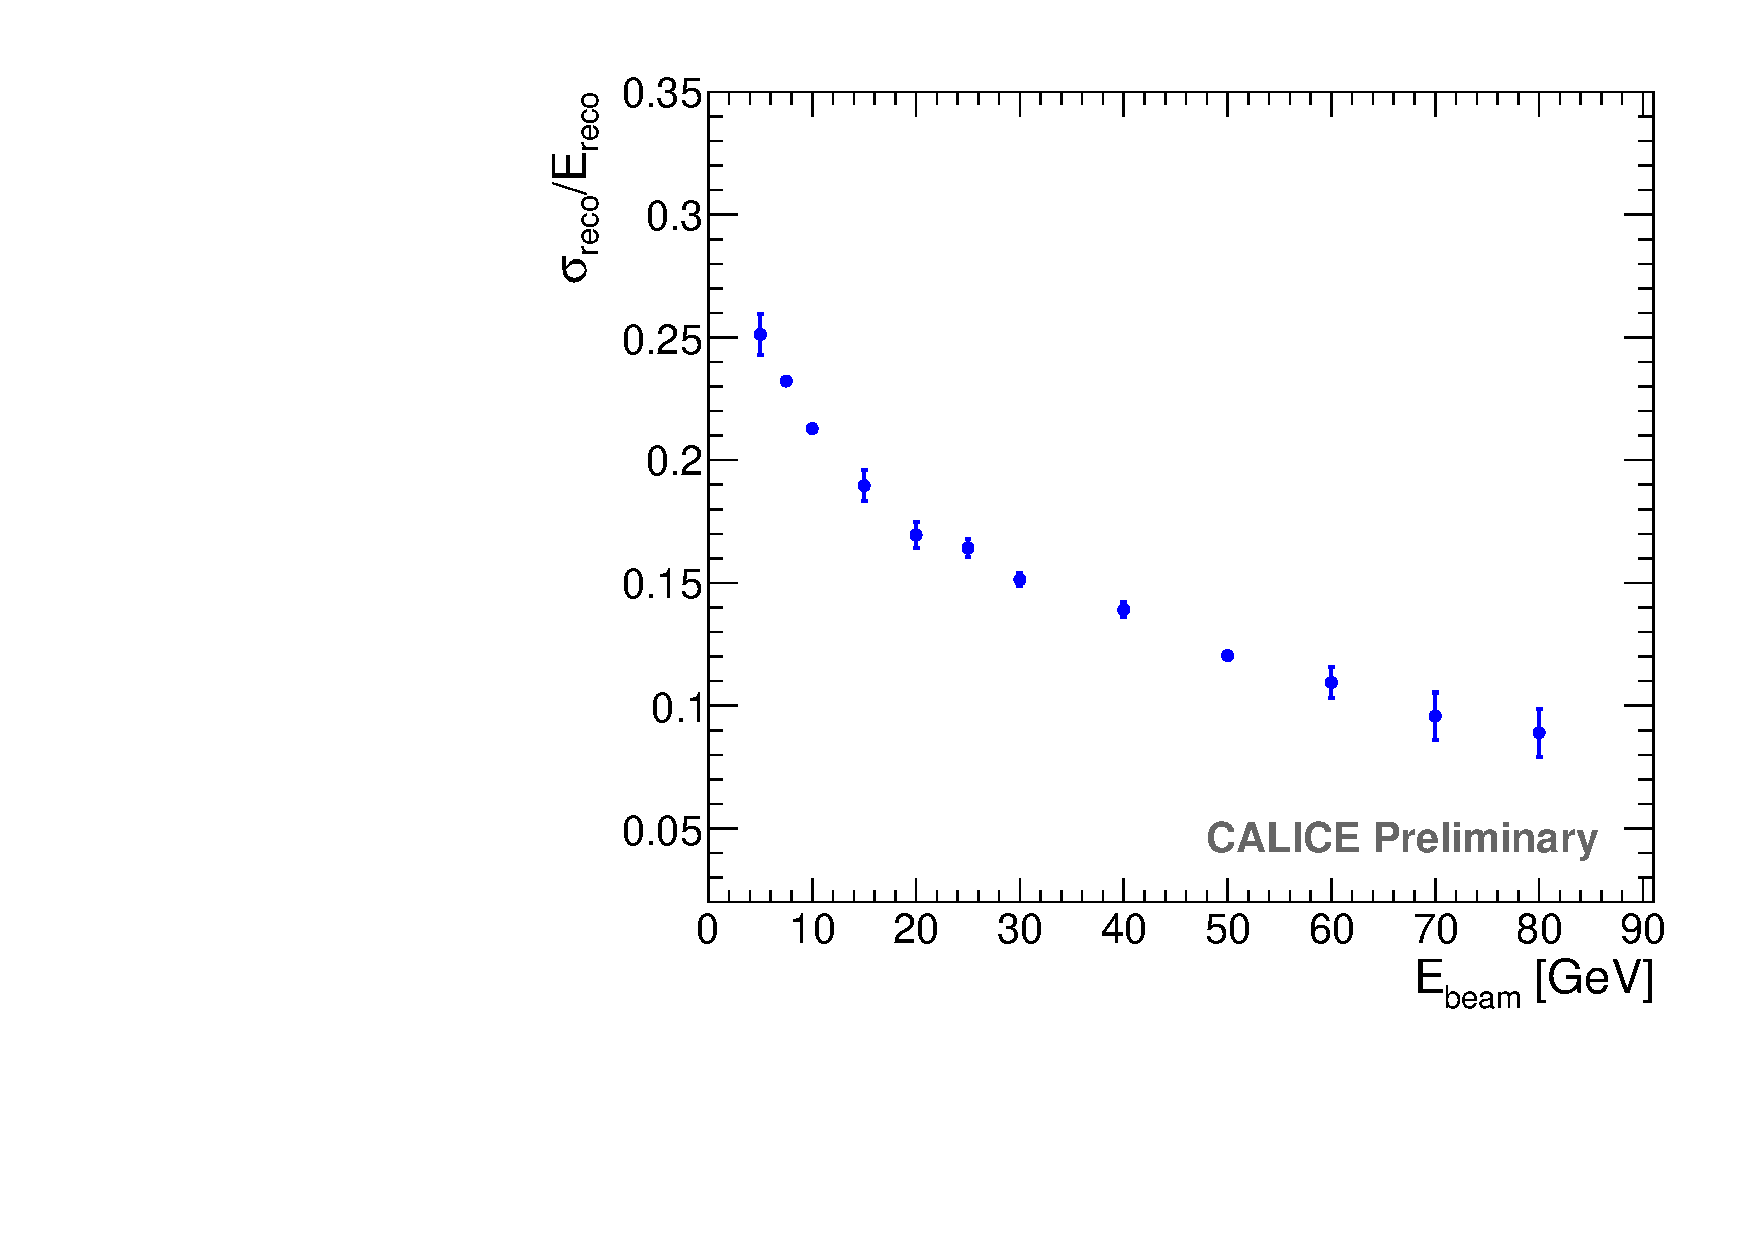
\includegraphics[width=\linewidth]{figs/Energy-Resolution.pdf}

        % \begin{center} The Calice Collaboration\\ JINST \textbf{11} P04001 \end{center}
      \end{center}
      \crefarticle{The Calice Collaboration}{JINST \textbf{11} P04001}
    \end{minipage}

  \end{frame}
\endgroup


\end{document}
